\documentclass[a4paper,12pt]{report}
\usepackage{graphicx}
\usepackage{titlesec}
\titleformat{\chapter}{}{}{0em}{\bf\LARGE}
\usepackage[utf8]{inputenc}
% Title Page
\title{Middle East Technical University\\Department of Physics\\PHYS222 Optics and Waves Laboratory\\\textbf{Experiment OW-5 Grating Spectrometer\\Laboratory Report}}

\author{Oğuzhan ÖZCAN\\1852334\\\\Partner: İnci SAİM\\\\Teaching Assistant: Hikmet ÖZŞAHİN}


\begin{document}
\maketitle
\tableofcontents
\listoffigures
\listoftables
\chapter{Theory}
A spectrometer is a very simple scientific instrument. It bends a light beam with a prism or diffraction grating. If light beam consist of more than one colours like white light beam then a spectrum is formed because various colour are reflected or diffracted to different colours. When a white light beam pass through spectrometer, we get an absoption spectrum since white light consist of all colours in visible spectrum. Theory of spectrometer is based on a simple fact. When an electron changes its orbit, light is emitted or absorbed. This is why we can use spectrometer while investigating the structure of atoms. Obviously, a spectrometer does not different from a prism. However, to be more precise in experiments, a spectrometer is more complicated. As seen in Figure 1.1, a spectrometer consist of three basic components; a collimator, a diffracting element and a telescope. The working principle of spectrometer is that the light enters to the collimator through a narraw slit which is positioned at focal point of collimator lens. The light beam leaves collimator as a thin and paralleled. Then the diffracting element or prism bends the beam of light. At this point if light consist of more than one colours, then we have a colour spectrum and besides each colour is diffracted to different angles. By rotating telescope, we can see different colour through eyepiece of spectrometer. By observing these specific colour spectrum we can determine the wavelength of corresponding colours [1].\\\\    
\begin{figure}[h]
\centering
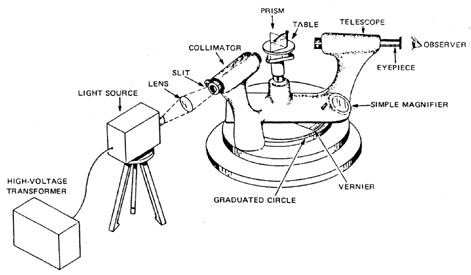
\includegraphics[width=0.9\linewidth, height=0.40\textheight]{spectrometer}
\caption{Student Type Grating Spectrometer}
\label{fig:spectrometer}
\end{figure}Although spectrometer is a simple instruments, it holds a very important optical phenomenon which known as \textit{diffraction grating}. A diffraction grating is one of the most useful devices to analyze light sources. Grating spectrometer is a similar device with Young's double slit experiment but grating spectrometer consist of much more slits. For instance, a typical grating has about 5000 grooves/cm and seperation between two slits is 1/5000 cm [2].\\\\
There are two types of diffraction gratings: \textit{transmission gratings} and \textit{reflection gratings}. Transmission gratings can be obtained by cutting parallel grooves on a glass
plate with a highly precise ruling machine. The spaces between the grooves act as
separate slits and produce transmitted interference fringes. On the other hand, reflection gratings can be obtained by cutting parallel grooves on a reflecting
surface with a highly precise ruling machine. The reflection of light from the
spaces between the grooves form the reflected interference fringes.\\\\
After giving definitions of gratings we need give some mathematical expressions. As we know a grating is an \textit{n}-slit system which is used in Fraunhofer diffraction. We can define grating equation as 
\begin{center}
	$m\lambda=d(\sin\theta+\sin\phi)$  
\end{center}
where \textit{m} is order number (\textit{m=0,1,2,3,...}) of the principal maxima, \textit{d} is the grating constant or spacing (distance between adjacent slits), $\phi$ is angle of incidence and $\theta$ is angle of diffraction. In most cases angle of incidence is 0 ($\phi=0$). Therefore we can define grating equation as 
\begin{center}
	$m\lambda=d\sin\theta$
\end{center}
Since the light is diffracted to different angles, we have to define the intensity distribution. Let consider \textit{N} is the number of slits and \textit{a} is the magnitude of grating. As we know light can act as an electromagnetic wave. When this wave diffracted the phase will change by equal amounts of $\delta$ from one slit to next [3] then the resultant complex amplitude of wave is 
\begin{center}
	$Ee^{i\theta}=a(1+e^{i\delta}+e^{2i\delta}+e^{3i\delta}+...+e^{i(N-1)\delta})=a\frac{1-e^{iN\delta}}{1-e^{i\delta}}$ 
\end{center}
To find the intensity we have multiply this equation by its complex conjugate.
\begin{center}
	$E^{2}=a^{2}\frac{(1-e^{iN\delta})(1-e^{-iN\delta})}{(1-e^{i\delta})(1-e^{-i\delta})}=a^{2}\frac{1-\cos N\delta}{1-\cos \delta}$
\end{center}
Using trigonometric properties of sine and cosine $1-\cos\alpha=2\sin^{2}(\alpha/2)$, we can write
\begin{center}
	$E^{2}=a^{2}\frac{\sin^{2}(N\delta/2)}{\sin^{2}(\delta/2)}=a^{2}\frac{\sin^{2}N\gamma}{\sin^{2}\gamma}$
\end{center}
where $\gamma=\lambda/2=(n\pi\sin\theta)/\lambda$. Now the factor $a^{2}$ represents the intensity diffracted by a single slit. Therefore we can define intensity of diffraction grating as
\begin{center}
	$I=E^{2}=E_{0}^{2}\frac{\sin^{2}\beta}{\beta^{2}}\frac{\sin^{2}N\gamma}{sin^{2}\gamma}$
\end{center}
At this point we have to define minima and secondary maxima. As we mentioned before $m\lambda=d\sin\theta$ is the principal maxima. To obtain minima we will use $1/N$ instead of $m$ because we have path difference. Therefore a minima for diffraction grating should be 
\begin{center}
	$d\sin\theta=\frac{\lambda}{N}, \frac{2\lambda}{N}, \frac{3\lambda}{N},...,\frac{(N-1)\lambda}{N}, \frac{(N+1)\lambda}{N},...$
\end{center}
One of the minor features of grating diffraction is the \textit{angular dispersion} \textit{D} which is the difference in angular position corresponding to a difference in wavelength. The angular dispersion can be defined as 
\begin{center}
	$D=d\theta/d\lambda$ 
\end{center}
Differentiating the grating equation yields
\begin{center}
	$D=m/(a\cos\theta_{m})$
\end{center}
This means that the angular seperation between two different frequency lines will increase as the order increases [4].\\\\
The Fraunhofer diffraction formula find important applications in the calculation of the \textit{resolving power} $\Re$ of optical systems. In a spectral apparatus the resolving power is a measure of the ability of the instrument to seperate two neighbouring spectral lines of slightly different wavelengths [5]. Resolving power can be defined as 
\begin{center}
{\Large 	$\Re=\frac{\lambda_{ave}}{\Delta\lambda}$  }
\end{center}
where $\lambda_{ave}=\lambda_{1}+\lambda_{2}/2$ and $\Delta\lambda=\lambda_{2}-\lambda_{1}$. If \textit{N} is the number of illuminated slits in the grating, then it can be shown that the
resolving power in the \textit{m}th-order diffraction which is 
\begin{center}
{\Large 	$\Re=mN$}
\end{center}












































\chapter{Data and Results}
\begin{table}[h]
	\begin{center}
\begin{tabular}{|c|c|}
	\hline Gas Discharge Lamb=  Mercury & Grating Spacing=1.66$\times10^{-3}$ mm \\ 
	\hline 
\end{tabular}
\end{center}
\caption{Properties of Grating Spectrometer}
\end{table} 
\begin{table}[h]
	\begin{center}
\begin{tabular}{|c|c|c|c|c|c|c|}
	\hline Color & $\theta^{\circ}_{Clockwise}$ & $\theta^{\circ}_{C-Clockwise}$ & $\theta^{\circ}_{Average}$ & $\lambda_{Calculated}$ & $\lambda_{Literature}$ & $\%$ Error\\  
	\hline White & $19^{\circ}$$0'$ & 0 & $9.5^{\circ}$ & 275.0 nm & None* & None \\ 
	\hline Violet & $14^{\circ}$$30'$ & $13^{\circ}$$42'$ & $14.1^{\circ}$ & 406.0 nm & 404.6 nm & 0.4 \\ 
	\hline Violet & $14^{\circ}$$36'$ & $13^{\circ}$$58'$ & $14.3^{\circ}$ & 411.2 nm & 407.8 nm & 0.8 \\ 
	\hline Blue & $15^{\circ}$$34'$ & $14^{\circ}$$58'$ & $15.3^{\circ}$ & 438.9 nm & 435.8 nm & 0.7 \\ 
	\hline Blue-Green & $17^{\circ}$$40'$ & $16^{\circ}$$23'$ & $17.0^{\circ}$ & 487.4 nm & 491.6 nm & 0.9 \\ 
	\hline Green & $19^{\circ}$$39'$ & $18^{\circ}$$55'$ & $19.3^{\circ}$ & 550.4 nm & 546.1 nm & 0.8 \\ 
	\hline Orange & $20^{\circ}$$50'$ & $19^{\circ}$$54'$ & $20.4^{\circ}$ & 580.0 nm & 577.0 nm & 0.5 \\ 
	\hline Orange & $20^{\circ}$$54'$ & $19^{\circ}$$8'$ & $20.0^{\circ}$ & 570.5 nm & 579.1 nm & 1.5 \\ 
	\hline 
\end{tabular} 
\end{center}
\caption{Experimental Data for Mercury Vapor Lamb}
\end{table} 
* White light does not have a certain wavelength. However, mercury vapor lamb produces a blueish white light [6] and blueish colour has a wavelength of 404.6 nm. Since percentage error would be very high, 31.9\%, this data is not useful.\\\\
\textbf{1. Determine the average values of $\theta$ for the observed spectral lines and fill them in \textit{Table 2.2.}}\\
\textbf{Note:} For an ideal adjusment, a given spectral line in a given order should occur at equal angles both to the left and to the right of central maximum. However, errors in the alignment of the grating may give rise to measurable differences. These errors will be largely cancelled by averaging the two values of $\theta$ obtained on either side of the central maximum.\\\\
\textbf{2. Using this information and $d\sin\theta=m\lambda$ equation, calculate the wavelengths of the spectral lines and fill your values in \textit{Table 2.2.}}\\\\
\textbf{3. Record the literature values of the wavelengths in \textit{Table 2.2} and complete the table by calculating the \% error.}\\\\
\textbf{4. Define the resolving power for grating spectrometers.}\\
The resolving power $\Re$ is proportional to the number of slits illuminated on the
diffraction grating. The resolving power also improves for higher diffraction
orders \textit{m}. Note that a spectrometer has relatively poor resolving power compared to a Fabry-Perot
interferometer [7]. The resolving
power of the diffraction grating is
\begin{center}
	$\Re \equiv\frac{\lambda}{\Delta\lambda}=mN$
\end{center}
\textbf{5. Calculate the theoretical resolving power of the grating spectrometer you have used in first, second and third order.}\\
Our spectrometer has 127 mm diameter and a 600 line/mm diffraction grating is available [8]. Therefore resolving power will be\\\\
\textit{For first order (m=1):}
\begin{center}
	$\Re=1\cdot$ 127 mm $\cdot$ 600 line/mm\\\framebox[80pt]{$\Re$=76200}
\end{center}
\textit{For second order (m=2):}
\begin{center}
	$\Re=2\cdot$ 127 mm $\cdot$ 600 line/mm\\\framebox[80pt]{$\Re$=152400}
\end{center}
\textit{For third order (m=3):}
\begin{center}
	$\Re=3\cdot$ 127 mm $\cdot$ 600 line/mm\\\framebox[80pt]{$\Re$=228600}
\end{center}
\textbf{6. What is the wavelength difference between two adjacent spectral lines that this spectrometer theoretically can resolve near 500 nm wavelength region?}\\
The minimum distinguishable wavelength seperation is 
\begin{center}
	{\Large $\Delta\lambda=\frac{\lambda}{\Re}$}
\end{center}
In the near 500 nm wavelength we will have The minimum distinguishable wavelength seperation for first order as 
\begin{center}
$\Delta\lambda$= 500 nm/76200\\
$\Delta\lambda=0.00656$ nm
\end{center}


















\chapter{Discussion and Conclusion}
\textbf{1.What are the possible errors in the experiment?}\\
The multiple reflections from the glass slides of the grating
introduce some error into the alignment procedure.
Normally, centering the cross-hairs between the reflected
images will reduce the error below the 1-minute resolution
that is obtainable when reading the vernier scales. Since we have very small percentage error, we can say that experimental errors are acceptable.\\\\
\textbf{2.What kind of approximation did you take into consideration while you were obtaining the physical quantities and how do they affect your results?}\\
Our Vernier Scale was wrong about 10'. While taking our data we considered this error and we made approximations about that. Small errors means that approximation that we took in the experiment do not effect negatively our results.\\\\
\textbf{3.What discrepancies did you encounter between the calculated quantities and theoretical or literature values?}\\
Obviously, we do not have certain discrepancies about experiment. Our experimental data is very close to theoretical values. It is certain that diffraction and reflection may cause error but these discrepancies are very small.\\\\ 
\textbf{4.What is your overall conclusion?}\\
To sum up, experiment is accomplished. We studied an important optical phenomena, diffraction grating and its related minors such as resolving power, angular dispersion etc. Besides, after this experiment we are more familiar with physical chemistry because these tools are widely using in physical chemistry and its applications.  
\chapter{Application}
\textbf{Radio Telescope}\\
One reason for building very large telescopes
is to increase the aperture diameter and thus
minimize diffraction effects. The effective
diameter of a telescope can be increased by
using arrays of smaller telescopes. The Very
Large Array (VLA) in New Mexico is a collection
of 27 radio telescopes, each 25 m in
diameter, that can be spread out in a Y-shaped
arrangement 36 km across. Hence the
effective aperture diameter is 36 km, giving
the VLA a limit of resolution of $5\times10^{-8}$ rad at a radio wavelength of 1.5 cm.
\begin{figure}[h]
\centering
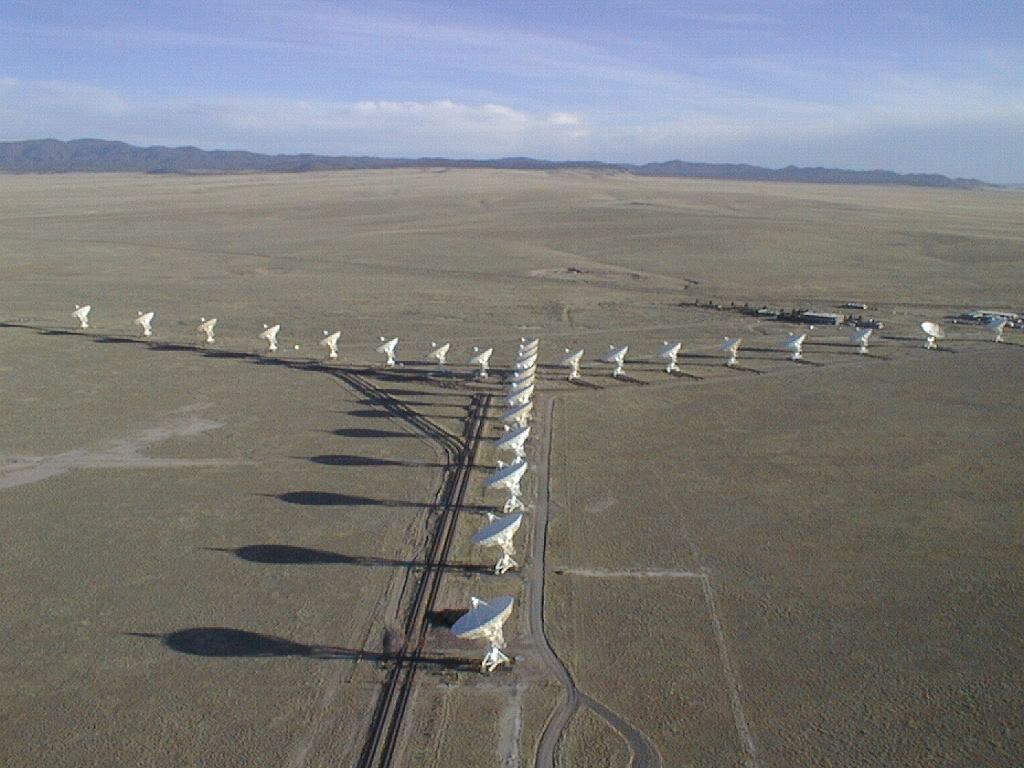
\includegraphics[width=0.7\linewidth, height=0.3\textheight]{vla}
\caption{NRAO Very Large Array}
\label{fig:vla}
\end{figure}
Radio telescope is an astronomical instrument consisting of a radio receiver and an antenna system that is used to detect radio-frequency radiation emitted by extraterrestrial sources. Because radio wavelengths are much longer than those of visible light, radio telescopes must be very large in order to attain the resolution of optical telescopes. The first radio telescope, built in 1937 by Grote Reber of Wheaton, Ill., U.S., was a steerable paraboloid--i.e., a device with a parabolically shaped reflector, dubbed the "dish," that focuses the incoming radio waves onto a small pickup antenna, or "feed." The radio telescope at Jodrell Bank, Cheshire, Eng., has a steerable paraboloid antenna 76 m (250 feet) in diameter (see photo above). The reflecting surface of the telescope at Arecibo, P.R., fills a naturally occurring bowl-shaped depression 305 m (1,000 feet) in diameter. Radio telescopes vary widely, but they all have two basic components: (1) a large radio antenna and (2) a radiometer or radio receiver. The sensitivity of a radio telescope--i.e., the ability to measure weak sources of radio emission--depends on the area and efficiency of the antenna, the sensitivity of the radio receiver used to amplify and detect the signals, and the duration of the observation. For broadband continuum emission the sensitivity also depends on the receiver bandwidth. Because some astronomical radio sources are extremely weak, radio telescopes are usually very large and only the most sensitive radio receivers are used. Moreover, weak cosmic signals can be easily masked by terrestrial radio interference, and great effort is taken to protect radio telescopes from man-made interference.\\\\
The most familiar type of radio telescope is the radio reflector consisting of a parabolic antenna--the so-called dish--which operates in the same manner as a television-satellite receiving antenna to focus the incoming radiation onto a small antenna referred to as the feed, a term that originated with antennas used for radar transmissions. In a radio telescope the feed is typically a waveguide horn and is connected to a sensitive radio receiver. Cryogenically cooled solid-state amplifiers with very low internal noise are used to obtain the best possible sensitivity.\\\\
Observing times up to many hours are expended and sophisticated signal-processing techniques are used to detect astronomical radio signals that are as much as one million times weaker than the noise generated in the receiver. Signal-processing and analysis are usually done in a digital computer. Although some of the computations may be carried out by microcomputers (i.e., those of the personal-computer class), other tasks require large, high-speed machines to translate the raw data into a form useful to the astronomer.\\\\
The performance of a radio telescope is limited by various factors: the accuracy of a reflecting surface that may depart from the ideal shape because of manufacturing irregularities; the effect of wind load; thermal deformations that cause differential expansion and contraction; and deflections due to changes in gravitational forces as the antenna is pointed to different parts of the sky. Departures from a perfect parabolic surface become important when they are a few percent or more of the wavelength of operation. Since small structures can be built with greater precision than larger ones, radio telescopes designed for operation at millimetre wavelength are typically only a few tens of metres across, whereas those designed for operation at centimetre wavelengths range up to 100 metres in diameter.\\\\
Some radio telescopes, particularly those designed for operation at very short wavelengths, are placed in protective radomes that can nearly eliminate the effect of both wind loading and temperature differences throughout the structure. Special materials that exhibit very low absorption and reflection of radio waves have been developed for such structures, but the cost of enclosing a large antenna in a suitable temperature-controlled radome may be almost as much as the cost of the movable antenna itself.\\\\
Radio telescopes are used to measure broad-bandwidth continuum radiation as well as spectroscopic features due to atomic and molecular lines found in the radio spectrum of astronomical objects. In early radio telescopes, spectroscopic observations were made by tuning a receiver across a sufficiently large frequency range to cover the various frequencies of interest. This procedure, however, was extremely time-consuming and greatly restricted observations. Modern radio telescopes observe simultaneously at a large number of frequencies by dividing the signals up into as many as several thousand separate frequency channels that may range over a total bandwidth of tens to hundreds of megahertz [9].











\chapter{References}
$[1]$ Born, M., \& Wolf, E. (1999). \textit{Principles of Optics: Electromagnetic Theory of Propagation, Interference and Diffraction of Light} (7th ed., p. 458). Cambridge: Cambridge University Press.\\
$[2]$ Radi, H., \& Rasmussen, J. (2013). \textit{Principles of Physics for Scientists and Engineers} (p. 320). Berlin: Springer.\\
$[3]$ Jenkins, F., \& White, H. (2001). \textit{Fundamentals of Optics} (4th ed., p. 337). New York: McGraw-Hill.\\
$[4]$ Hecht, E. (2002). \textit{Optics} (4th ed., p. 480). Reading, Mass.: Addison-Wesley.\\
$[5]$ Kenyon, I. (2008). \textit{The Light Fantastic: A Modern Introduction to Classical and Quantum Optics} (pp. 139,141). Oxford England: Oxford University Press.\\
$[6]$ Schiler, M. (1992). \textit{Simplified Design of Building Lighting} (p. 27). New York: Wiley.\\
$[7]$  Peatross, J., \& Ware, M. (2014). \textit{Physics of Light and Optics} (2013 ed., p. 285). Provo, UT: Brigham Young University Press.\\
$[8]$ Student Spectrometer Instruction Manual. (2003, October 1). Retrieved April 27, 2015, from http://www.pasco.com/file-downloads/product-manuals\\/Student-Spectrometer-Manual-SP-9268A.pdf\\
$[9]$ Radio Telescope. (n.d.). Retrieved April 27, 2015, from http://abyss.uoreg\\on.edu/~js/glossary/radio-telescope.html


























































































\end{document}          
